\documentclass{ctexart}
\usepackage{fancyhdr}
\usepackage{amsmath}
\usepackage{indentfirst}
\usepackage{cjkindent}
\usepackage{graphicx}
\pagestyle{fancy}
\lfoot{}%这条语句可以让页码出现在下方
\title{《算法设计与分析》\\ 第二次作业} 
\author{\\姓名:曹建钬 \\  \\
学号:20375177}
\date{}
\usepackage[ruled,vlined,linesnumbered,lined,commentsnumbered]{algorithm2e}

\begin{document}
\pagestyle{empty}
\thispagestyle{empty}
\CTEXsetup[format={\Large\bfseries}]{section}
\maketitle
\clearpage

\section{小跳蛙问题}


\subsection{Main Idea}
小跳蛙从第1块跳至第$n$块石头上,最后一跳的起跳点一定位于第$(n-k)$、$(n-k+1) \ldots (n-1)$块石头,而子问题是重叠的,因此可以使用动态规划方法进行解题。

令$MSC(n)$为小跳蛙从第$1$块石头跳至第$n$块石头最少耗费的体力,那么有递推关系:
\begin{align*}
    MSC(n) = Min\{MSC(n-1)+|h_n-h_{n-1}|\\
    MSC(n-2)+|h_n-h_{n-2}| \\
    \ldots \\
    MSC(n-k)+|h_n-h_{n-k}|
    \}
\end{align*}
算法的伪代码如下:
\subsection{Pseudo Code}

\begin{algorithm}[H]
    \SetAlgoLined %显示end
	\caption{$Minimum-Strength-Cost(n,H,k)$}%算法名字
	\BlankLine
	\KwIn{石头数量$n$,从第$1$块到第$n$块石头的高度$h_i$组成的数组$H$,青蛙最远跳跃距离$k$}%输入参数
	\KwOut{从第一块石头跳至第$n$块石头耗费的最少体力}%输出
	\BlankLine
	\tcp{初始化}
	创建一维数组$MSC[1\ldots n]$ \;
	$MSC[1] \leftarrow 0$ \; 
	\tcp{$MSC[i]$为小跳蛙从第$1$块跳至第$i$块石头最少耗费的体力}
	\For{$i \leftarrow 2$ to $n$}
	{\For{$j \leftarrow 1$ to $Min(k,i-1)$}{	
	$MSC[i] \leftarrow Min(MSC[i-j]+|h_i-h_{i-j}|)$}}
	\textbf{return $MSC[n]$}
\end{algorithm}

\subsection{Complexity Analysis}
算法的时间复杂度$T(n,k)$来自于4-8行的双重循环,以比较为基本运算,故有
\begin{align*}
    T(n,k) = O(n \cdot k)
\end{align*}

\section{二进制串变换问题}


\subsection{Main Idea}
分析题目,对字符串$a$只能进行以下两种操作:
\begin{enumerate}
    \item 交换$a_i$和$a_j$,操作代价为$|i-j|$
    \item 取反$a_i$,操作代价为$1$
\end{enumerate}

交换两个不同的字符除了使用操作1实现,还可以对这两个字符分别进行取反,即进行两次操作2。因此,如果两个不同的字符不相邻($i-j \geq 2$),使用操作2更优,相邻的情况即可进行交换以将操作代价减小为1。

此题与最小编辑问题类似,这里同样使用动态规划进行解题:

令$C[i]$为$a[1 \ldots i]$变为$b[1 \ldots i]$所需的最小代价,递推关系如下:
\begin{itemize}
    \item 若$a[i] = b[i]$则:$C[i]=C[i-1]$
    \item 若$a[i] \neq b[i]$则:
    \begin{itemize}
        \item 当$a[n-1]=b[n]$且$a[n]=b[n-1]$:$C[i]=C[i-2]+1$
        \item 其余情况:$C[i]=C[i-1]+1$
    \end{itemize}
\end{itemize}
算法的伪代码如下:
\subsection{Pseudo Code}

\begin{algorithm}[H]
    \SetAlgoLined %显示end
	\caption{$Operation-Cost(a,b,n)$}%算法名字
	\BlankLine
	\KwIn{长度为$n$的仅由0和1组成的字符串$a$和$b$}%输入参数
	\KwOut{将串$a$变为串$b$的最小代价}%输出
	\BlankLine
	\tcp{初始化}
	创建一个一维数组$C[0\ldots n]$ \;
	$C[0] \leftarrow 0$ \;
	\eIf{$a[1] \neq b[1]$}{$C[1] \leftarrow 1$}{$C[1] \leftarrow 0$}
	\tcp{$C[i]$代表$a[1 \ldots i]$变为$b[1 \ldots i]$所需的最小代价}
	\For{$i \leftarrow 2 $ to $n$}
	{
	\eIf{$a[i]=b[i]$}{$C[i]=C[i-1]$}
	{
	\eIf{$a[n-1]=b[n]$ and $a[n]=b[n-1]$}{$C[i]=C[i-2]+1$}{$C[i]=C[i-1]+1$}
	}
	}
	\textbf{return $C[n]$}
\end{algorithm}

\subsection{Complexity Analysis}
令算法的时间复杂度为$T(n)$,以比较判断为基本运算,从伪代码中可以看出,$C[1]$只需要一次判断即可得到,而$C[2]$到$C[n]$每个则需要进行3次判断,则有:
\begin{align*}
   T(n)=1+3(n-1)=O(n) 
\end{align*}

\section{球队组建问题}

\subsection{Main Idea}
分析此问题可作出如下形式化定义:
\begin{itemize}
    \item 输入:序列$A=<h_{1,1},h_{1,2},\ldots,h_{1,n}>$和序列$B=<h_{2,1},h_{2,2},\ldots,h_{2,n}>$
    \item 输出:求解一个由序列$A$和序列$B$中元素组成的新序列$N=<h_1,h_2,\ldots,h_z>$使得$\sum_{i=1}^{i=z} h_i$最大。
    \item 约束条件:不能同时选择$A$中的$h_{1,k}$和$B$中的$h_{2,k}$,且各序列中的相邻元素不能同时被选(比如:选择了$A$中的$h_{1,k}$就不能选择$h_{1,k-1}$和$h_{1,k+1}$)
\end{itemize}


可能存在最优子结构和重叠子问题,故利用动态规划的思想。以$H[j]$代表由$A<h_{1,1},h_{1,2},\ldots,h_{1,j}>$和$B<h_{2,1},h_{2,2},\ldots,h_{2,j}>$中元素构成的最高队列的高度。

如下图所示,在队列$A$和队列$B$中截取紧挨着的前三列($j=3$的情况下),只存在以下四种基本情况可能成为这三列中的最优解。
从中可以看出:末尾元素:$h_{1,j}$和$h_{2,j}$中一定有且只有一个元素被选中(否则一定不是最优解),而且可能存在夹在非空列之间的空列。

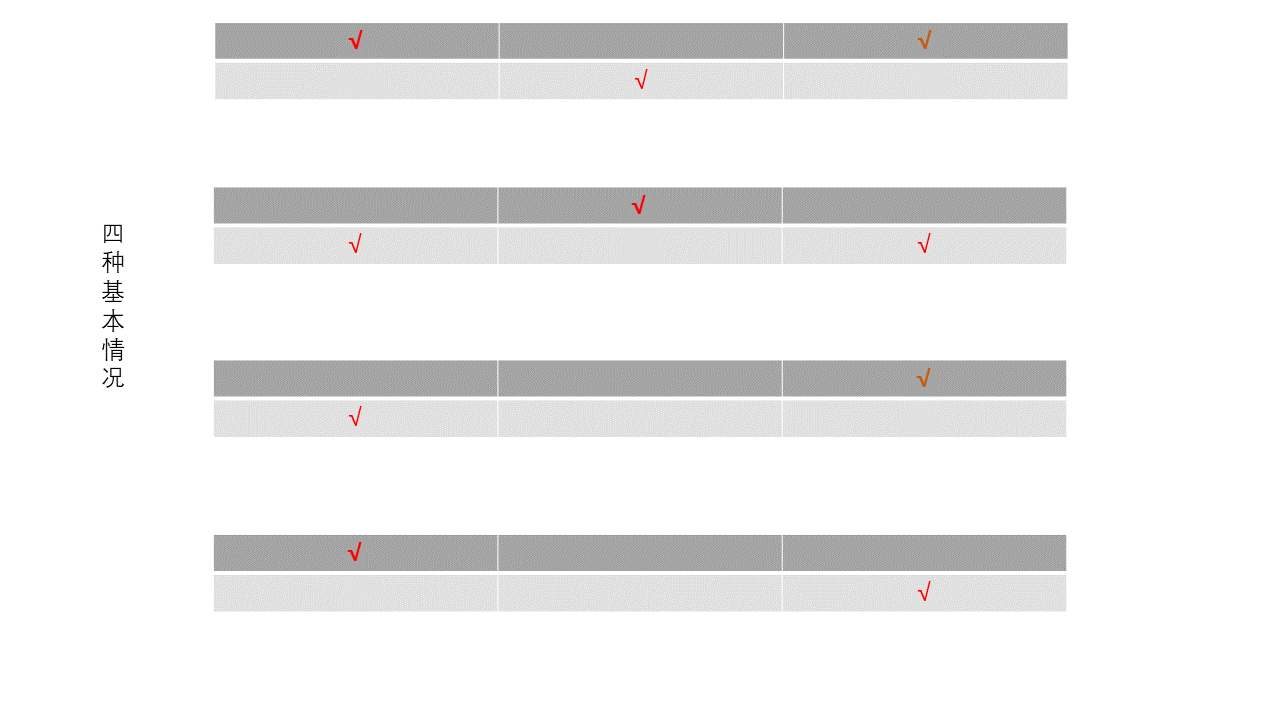
\includegraphics[width=1.0\textwidth]{幻灯片1.PNG}

那么有没有可能出现两列同时没被选呢?从下图($j=4$的情况)可以看出,一旦出现这种情况,那么其一定不是最优解。因此$H[j]$最优解存在最优子结构:要不从$H[j-2]$中隔一行得到,要不从$H[j-1]$中得到。

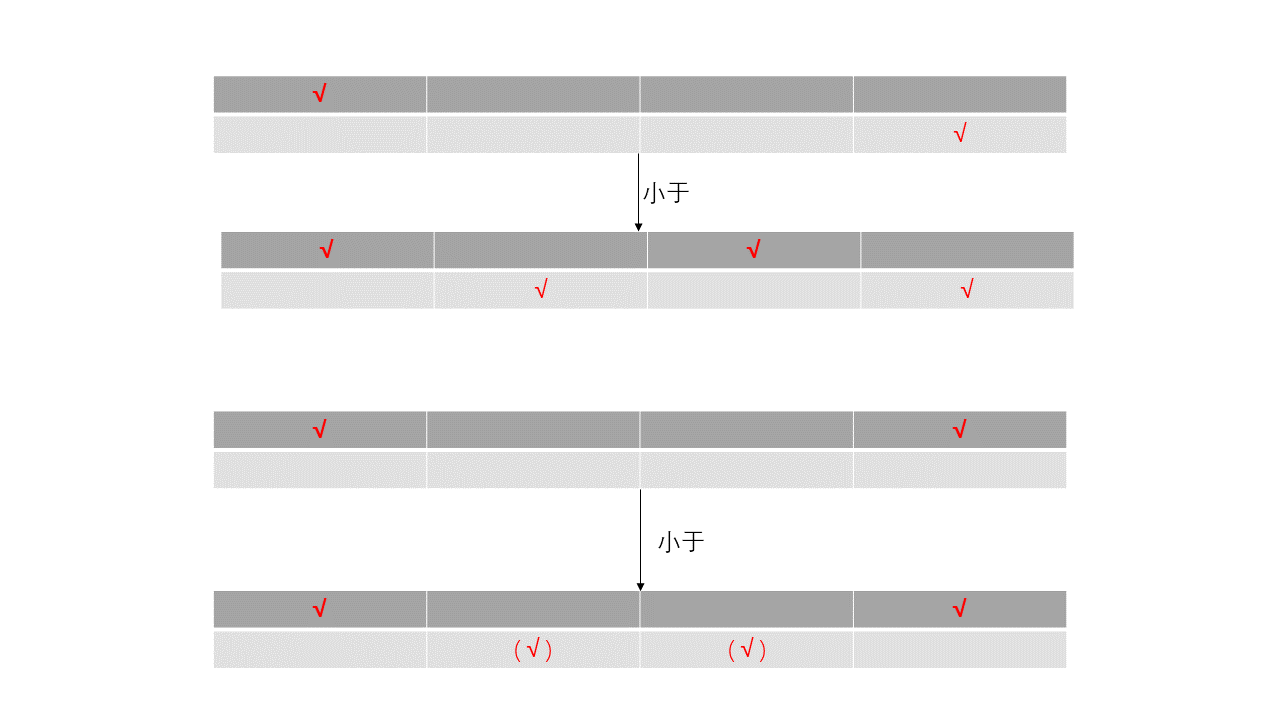
\includegraphics[width=1.0\textwidth]{幻灯片2.PNG}

为了便于描述递推关系,将$H[j]$根据最后的元素的来源分为上下两种情况,以$H[1,j]$表示代表取$h_{1,j}$时,由$A<h_{1,1},h_{1,2},\ldots,h_{1,j}>$和$B<h_{2,1},h_{2,2},\ldots,h_{2,j}>$中元素构成的最高队列的高度,以$H[2,j]$表示代表取$h_{2,j}$时,由$A<h_{1,1},h_{1,2},\ldots,h_{1,j}>$和$B<h_{2,1},h_{2,2},\ldots,h_{2,j}>$中元素构成的最高队列的高度,则有$H[i]=\max(H[1,j],H[2,j])$,同时可得以下递推关系:
\begin{itemize}
    \item $H[1,j]=\max(H[2,j-2]+h_{1,j}\ ,\ H[2,j-1]+h_{1,j})$
    \item $H[2,j]=\max(H[1,j-1]+h_{2,j}\ ,\ H[1,j-2]+h_{2,j})$
    \item $H[i]=\max(H[1,j],H[2,j])$
\end{itemize}

过程如下图所示:

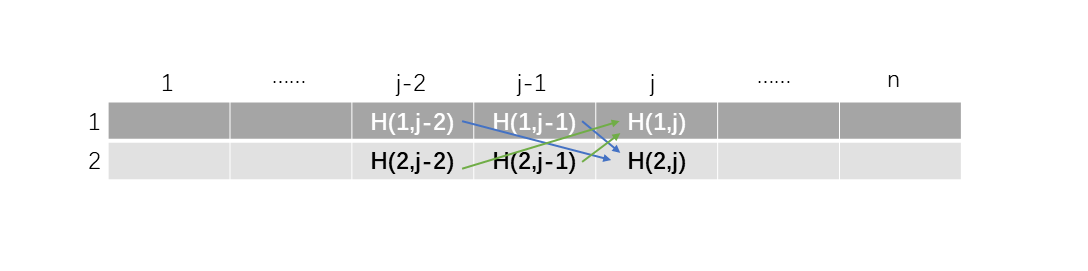
\includegraphics[width=1.0\textwidth]{final.PNG}

记录决策过程:

$$Rec[i,j]=\left\{
\begin{aligned}
& 1   & if \ choose \ h_{3-i,j-1}\\
& 2   & if \ choose \ h_{3-i,j-2} 
\end{aligned}
\right.
$$

其中$i$取1或2,$3-i$即为第$i$行的相邻行,$2 \leq j \leq n$,伪代码如下:



\subsection{Pseudo Code}

\begin{algorithm}[H]
    \SetAlgoLined %显示end
	\caption{$HighestQueue(h_{i,j})$}%算法名字
	\BlankLine
	\KwIn{同学们的身高数据$h_{i,j}$,$h_{1,j}$($1 \leq j \leq n$)表示第一排同学的身高,$h_{2,j}$($1 \leq j \leq n$)表示第二排同学的身高}%输入参数
	\KwOut{组建成的球队中成员的身高之和最大的方案}%输出
	\BlankLine
	\tcp{初始化}
	创建二维数组$H[1..2,1..n]$和$Rec[1..2,2..n]$ \\
	$H[1,1] \leftarrow h_{1,1}$ \\
	$H[2,1] \leftarrow h_{2,1}$ \\
	$H[1,2] \leftarrow h_{2,1}+h_{1,2}$ ,$Rec[1,2] \leftarrow 1$ \\
	$H[2,2] \leftarrow h_{1,1}+h_{2,2}$ ,$Rec[2,2] \leftarrow 1$ \\
	\tcp{求解表格}
	\For{$j \leftarrow 3 \ to\  n $}
	{
	\For{$i \leftarrow 1 \ to\  2 $}
	{
	\eIf{$H[3-i,j-2] > H[3-i,j-1]$}{$H[i,j]\leftarrow H[3-i,j-2]+h_{1,j}$ \\ $Rec[i,j] \leftarrow 2$}{$H[i,j]\leftarrow H[3-i,j-1]+h_{1,j}$ \\ $Rec[i,j] \leftarrow 1$}
	}
	}
	\tcp{输出最优方案}
	$j \leftarrow n$ \\
	$i \leftarrow \max_{i=1,2}(H[i,n])$ \\
	print 第$i$排第$n$个学生被选中 \\
	\While{$j > 1$}
	{
	$j \leftarrow j-Rec[i,j]$ \\
	$i \leftarrow 3-i$ \\
		print 第$i$排第$j$个学生被选中 \\
	}
\end{algorithm}

\subsection{Complexity Analysis}
令算法的时间复杂度为$T(n)$,$n$为每一排学生的人数,以比较大小为基本运算,复杂度主要来源于8-18行的循环,则有:
\begin{align*}
    T(n)=O(n)
\end{align*}
\section{括号匹配问题}

\subsection{Main Idea}
问题定义:
\begin{itemize}
    \item 输入:由‘[’,‘]’和‘(’,‘)’构成的长度为$n$的字符串$str[1\ldots n]$
    \item 输出:该串中合法子序列的最大长度
\end{itemize}

以$L[i,j]$表示子字符串$str[i \ldots j]$的最长合法子序列的长度。
则原始问题为:$L[1,n]$,即计算字符串$str[1 \ldots n]$的最长合法子序列的长度。其中$1 \leq i \leq j \leq n$

寻找最优子结构和递推关系:
\begin{itemize}
    \item $str[i]$与$str[j]$匹配时:$L[i,j] = L[i+1,j-1]+2$
    \item $str[i]$与$str[j]$不匹配时:
    \begin{equation*}
        L[i,j]=\max_{i \leq k < j}(L[i+1,j-1],L[i,k]+L[k+1,j])
    \end{equation*}
\end{itemize}


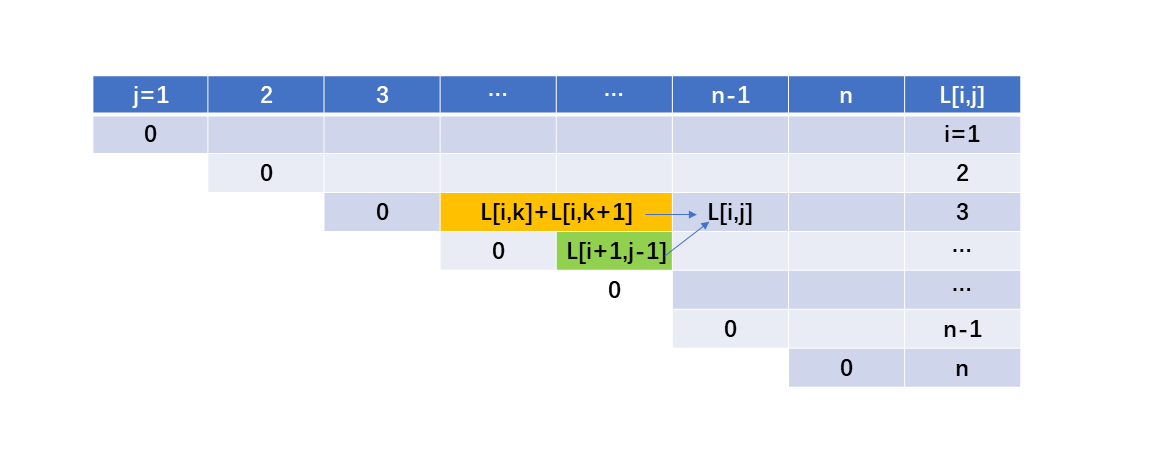
\includegraphics[width=1.1\textwidth]{幻灯片3.PNG}

自底向上确定计算顺序:

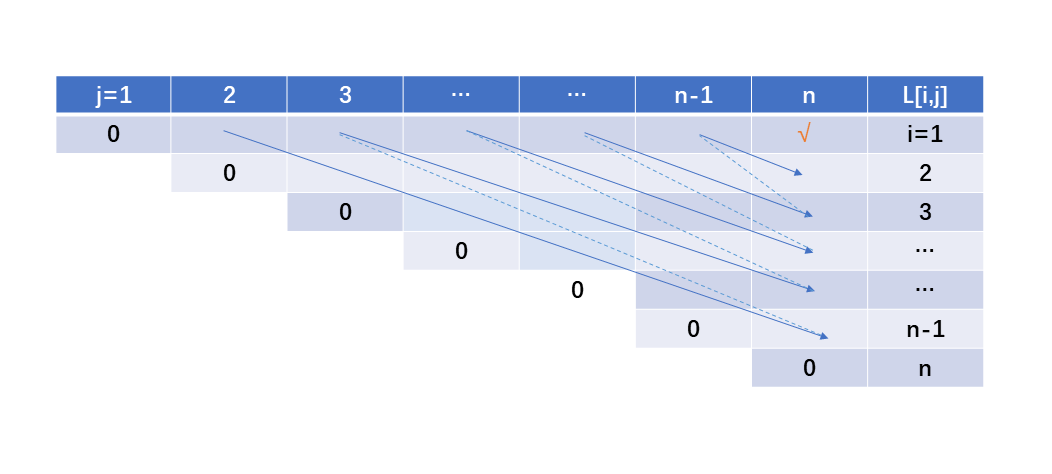
\includegraphics[width=1.1\textwidth]{幻灯片5.PNG}

逆时针旋转45度,如下图所示:

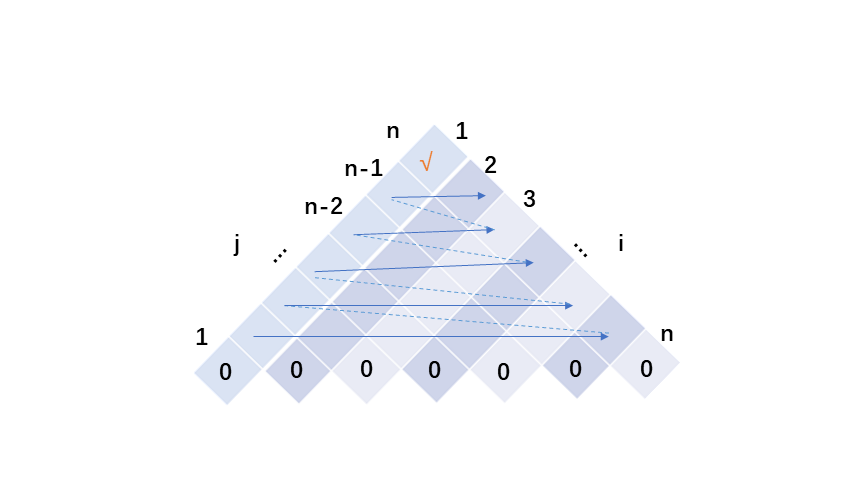
\includegraphics[width=1.1\textwidth]{幻灯片4.PNG}

伪代码如下:

\subsection{Pseudo Code}

\begin{algorithm}[H]
    \SetAlgoLined %显示end
	\caption{$Longest-Legal-Subsequences(str)$}%算法名字
	\BlankLine
	\KwIn{字符串$str$}%输入参数
	\KwOut{$str$的最长合法子序列的长度}%输出
	\BlankLine
	$n \leftarrow length(str)$ \\
	\tcp{初始化}
	新建二维数组$L[1 \ldots n]$ \\
	\For{$i \leftarrow 1\  to\  n$ }{$L[i,i] \leftarrow 0$}
	\tcp{动态规划,其中$l$代表区间长度}
    \For{$l \leftarrow 2\ to \ n$ }
    {
    \For{$i \leftarrow 1 \ to \ n-l+1$}
    {
    $j \leftarrow i+l-1$ \\
    \eIf{$str[i]$与$str[j]$相匹配}{$L[i,j] \leftarrow L[i+1,j-1]+2$}
    {
    \For{$k \leftarrow i \ to \ j-1$}
    {
    $L[i,j] \leftarrow \max(L[i,k]+L[k+1,j],L[i+1,j-1])$
    }
    }
    }
    }
	\textbf{return $L[1,n]$}
\end{algorithm}


\subsection{Complexity Analysis}

以$T(n)$代表此算法的时间复杂度,$n$为原字符串的长度,以一次大小的比较为基本运算。根据8-19行,最坏的情况下需要经历三重循环,则有:
\begin{align*}
    T(n) = O(n^3)
\end{align*}

\section{箱子问题}

\subsection{Main Idea}
此问题很像$LIS$问题,但箱子问题中要想一个箱子$A$要水平地放在另一个箱子$B$上,要求箱子$A$底面的长和宽都严格小于箱子$B$。这涉及到两个量的比较,这里以底面积大小为标准将箱子从大到小进行排序,一个底面积大的箱子永远不能出现在底面积小的箱子上面,但是底面积小的箱子可以或不能出现在底面积大的箱子上面,这样就可以在减小计算量的同时不落下每一种可能的情况。

需要注意的是,箱子可以任意进行旋转,那么$n$中箱子中的每一种箱子$a_i$(高$h_i$宽$w_i$长$d_i$)最多可产生三种不同底面积的箱子:$h_i * w_i$、$h_i * d_i$、$w_i * d_i$,每一种均需要参与排序和选择,问题的规模最大为$3n$,下面只考虑最大规模的情况。

寻找最优子结构和递推关系,此问题最优解依赖枚举子问题,与课上所讲的钢条切割问题类似,以$MTH[j]$代表以第$j$种箱子为塔顶时塔的最大高度,有如下递推关系:
\begin{itemize}
    \item $i$从$1$遍历至$j-1$,对于每一种满足$width(j)<width(i)$和$depth(j)<depth(i)$的可能:
    \begin{align*}
    MTH[j] = \max(MTH[i]) + height(j)
\end{align*}
    \item 遍历完成后,如果没有一个$i$使得$width(j)<width(i)$和$depth(j)<depth(i)$:
    \begin{align*}
    MTH[j] = height(j)
\end{align*}
\end{itemize}


为了求出最优的建塔方案,还需要构造追踪数组$rec[1 \ldots 3n]$,用$rec[j]$记录以第$j$种箱子为顶的最高建塔方案。其中:
\begin{itemize}
    \item $rec[j]=j$:以第$j$种箱子为最底层
    \item $rec[j]=i$:以第$j$种箱子为上层,而下层为$rec[i]$建塔方案
\end{itemize}

伪代码如下:
\subsection{Pseudo Code}

\begin{algorithm}[H]
    \SetAlgoLined %显示end
	\caption{$Maximum-Tower-Height(a,n)$}%算法名字
	\BlankLine
	\KwIn{$n$种箱子,且$a_j=\{h_j,w_j,d_j\}$}%输入参数
	\KwOut{使得该塔的高度最高的建塔方案}%输出
	\BlankLine
	\tcp{初始化}
	新建一维数组$MTH[1 \ldots 3n]$和$rec[1 \ldots 3n]$ \\
	\For{$j \leftarrow 1 \ to \ n$}
	{$rot[3j-2] \leftarrow \{h_j,w_j,d_j\}$ \\
	 $rot[3j-1] \leftarrow \{w_j,h_j,d_j\}$ \\
	 $rot[3j] \leftarrow \{d_j,w_j,h_j\}$ } 
	$rot[1 \ldots 3n]$按底面积大小($rot[j][2]*rot[j][3]$)进行降序排序\\
	\tcp{动态规划,其中$MTH[best]$为最高高度}
	$best \leftarrow 1$ \\
	\For{$j \leftarrow 1 \ to \ 3n$}{$rec[j] \leftarrow j$ \\ $MTH[j] \leftarrow rot[j][1]$\\
	\For{$i \leftarrow 1 \ to \ j-1$}
	{
	\If{ $rot[j][2] < rot[i][2]$\  and \ $rot[j][3] < rot[i][3]$}{\If{$MTH[i]+rot[j][1] > MTH[j]$}{$MTH[j] \leftarrow MTH[i]+rot[j][1]$ \\ $rec[j] \leftarrow i$}}
	}
	\If{$MTH[best] < MTH[j]$}{$best \leftarrow j$}
	
	}
    \tcp{输出最优方案}
	$cal \leftarrow 1 $ \\
	print 第$cal$层放置以$rot[best][2]*rot[best][3]$为底面的箱子,该箱子的高度为$rot[best][1]$ \\
	\While{$rec[best] \leq best$}
	{
	$cal \leftarrow cal+1$ \\
	print 第$cal$层放置以$rot[rec[best]][2]*rot[rec[best]][3]$为底面的箱子,该箱子的高度为$rot[rec[best]][1]$ \\
    $best \leftarrow rec[best]$
	}

\end{algorithm}

\subsection{Complexity Analysis}
以$T(n)$代表此算法的时间复杂度,$n$为给定的箱子的种数。

第3-7行需要循环遍历$n$次复杂度为$O(n)$,第8行降序排序复杂度为$O(nlogn)$,第11-25行双重循环复杂度为$O(n^2)$。综上:
\begin{align*}
    T(n)=O(n^2)
\end{align*}


\end{document}